\documentclass[letterpaper]{article} % DO NOT CHANGE THIS

% ============================================================
% NeurIPS 2026 workshop style, camera-ready (non-archival).
% `final` de-anonymises, drops line numbers and sets the workshop footer.
% NEmo asks for sglblindworkshop.  Under `final` it renders the same as
% dblblindworkshop (neurips_2026.sty:85-93).
% ============================================================
\usepackage[final,sglblindworkshop]{neurips_2026}
\usepackage[hyphens]{url}          % DO NOT CHANGE THIS
\usepackage{graphicx}              % DO NOT CHANGE THIS
\usepackage{caption}               % DO NOT CHANGE THIS
% Additional packages used in this paper
\usepackage{amsmath}
\usepackage{amssymb}
\usepackage{booktabs}
\usepackage{multirow}
\usepackage{microtype}
\usepackage{array}
\usepackage{pifont}
\usepackage{tikz}
\usetikzlibrary{positioning,arrows.meta,fit,backgrounds}
% The official NeurIPS 2026 template loads hyperref too; here it comes last,
% after caption and tikz.  It gives clickable links and PDF metadata, and
% hidelinks keeps the look of the reviewed version.  Keep pdftitle equal to
% \title: check_format.py --final compares them.
\usepackage[hidelinks]{hyperref}
\hypersetup{pdfauthor={Zixuan Wang, Ziming Dai, Yu Wu, Li Ning}}
\hypersetup{pdftitle={Existence Before Relevance: Same-Category
  Demonstrations Narrow a Prerequisite-Chain Gap in LLM Plan Generation, and
  Pass On Their Defects}}

% booktabs breathing room.  neurips_2026.sty:238 swaps above/belowcaptionskip
% for tables, but \usepackage{caption} redefines \@makecaption and ignores it,
% so a table caption lands flush on \toprule.  \abovetopsep restores the gap;
% the rulesep pair keeps header/body off the rules.
\setlength{\abovetopsep}{6pt}
\setlength{\aboverulesep}{0.6ex}
\setlength{\belowrulesep}{0.8ex}

% neurips_2026.sty:145 sets \flushbottom.  Whenever a page cannot be filled --
% which happens on every page that defers a tall appendix table -- \flushbottom
% pays for the shortfall out of the only stretchable glue available:
% \textfloatsep and the \section skips.  The result is several cm of white
% smeared between a heading and its first paragraph.  \raggedbottom parks the
% slack at the page foot instead, where nothing looks broken.
\raggedbottom

% Same idea for float pages.  LaTeX's defaults (\@fptop/\@fpsep/\@fpbot all
% carry 1--2fil) centre and spread the floats, so a two-table page reads as two
% tables adrift in white.  Pin them to the top, fixed gap, slack to the foot.
\makeatletter
\setlength{\@fptop}{0pt}
\setlength{\@fpsep}{18pt}
\makeatother


% cross-reference helpers: never hardcode section numbers
\newcommand{\secref}[1]{\S\ref{#1}}
% The appendices are a separate document, MCAI_neurips_ws_appendix.tex, so
% their numbers come from its .aux through xr.  \getrefnumber prints the number
% as plain text, because a link to another PDF has no target here.  An unknown
% label prints UNRESOLVED, which check_format.py rejects.
\usepackage{xr}
\usepackage{refcount}
\setrefcountdefault{UNRESOLVED}
\externaldocument{MCAI_neurips_ws_appendix}
\newcommand{\appref}[1]{Appendix~\getrefnumber{#1}}

% convenience macros for significance stars
\newcommand{\sigC}{$\star\!\star\!\star$}
\newcommand{\sigB}{$\star\!\star$}

\title{Existence Before Relevance: Same-Category Demonstrations Narrow a
       Prerequisite-Chain Gap in LLM Plan Generation, and Pass On Their Defects}
\workshoptitle{Neuro-Symbolic Embodied Intelligence}
% Names, order, affiliations and emails were given by the author (2026-10-31).
\author{%
  Zixuan Wang$^{1}$\quad Ziming Dai$^{2}$\quad Yu Wu$^{3}$\quad Li Ning$^{4}$ \\
  $^{1}$Shenzhen College of International Education\quad
  $^{2}$BASIS International Schools \\
  $^{3}$CuliuTech\quad
  $^{4}$Stellaris AI Limited \\
  \texttt{\small zw6963470@gmail.com}\quad \texttt{\small benjamin.dai66@gmail.com} \\
  \texttt{\small wuyu@culiu-tech.com}\quad \texttt{\small lining@stellaris-ai.com}
}

\begin{document}
\maketitle

% ============================================================
\begin{abstract}
Large language models (LLMs) are increasingly used as task planners for
embodied agents, yet long prerequisite chains remain a weak point.  We study
this in offline plan generation for a Minecraft agent, scoring each plan with
a rule-based validator that walks it over a virtual inventory.  For five of
the seven LLMs we test (8B to 671B parameters where disclosed), plans for
two-chain (L2) tasks pass only 10--30\% of the time without retrieval, against
45--95\% on single-material tasks.  Adding three same-category demonstrations
to the prompt improves all five.  In a four-condition ablation on one model,
randomly chosen same-category demonstrations recover most of the gain ($+$31
percentage points; $+$20 when the scorer also charges consumed materials), and
ranking them by relevance over the game's recipe graph adds a smaller increment
over lexical ranking ($+$12 points) that neither our pre-specified correction
nor the stricter scorer confirms.  Demonstration content is also inherited
verbatim: an invalid command in the combat demonstrations appears in 71.5\% of
retrieval trials on those tasks and in none of 505 trials without retrieval.
In this setting, adding same-category demonstrations to a shared rule text
matters more than selecting them precisely, and their defects have to be
checked because they are copied.
\end{abstract}

% ============================================================
\section{Introduction}
\label{sec:intro}

An LLM that plans for a virtual embodied agent needs long chains of
procedural, version-specific knowledge:
which tool mines which block, what a recipe consumes, which intermediate item
must exist first.  A symbolic planner is handed this knowledge as a domain
model; an LLM planner is assumed to have absorbed it in pretraining.
Minecraft makes the difference measurable.  Frontier models decompose
single-step goals readily~\citep{wang2023voyager,wang2023describe}, and
Plancraft~\citep{dagan2024plancraft} finds that they struggle with multi-step
crafting.  We ask which facet of that knowledge an LLM planner must be
\emph{given} rather than assumed to hold: its existence in the prompt as worked examples, its
relevance to the query, its correctness, or the model's capacity to use it.

\textbf{Scope.}  This is a study of LLM \emph{plan generation} with an
embodied motivation.  Every confirmatory result comes from scoring generated
plans offline: a rule-based validator walks each plan over a virtual inventory
whose initial state is given by construction, with no perception, symbol
grounding or execution.  A live-execution study does not separate the
conditions and is reported as a limitation, not as evidence
(\secref{sec:limits}).  The neuro-symbolic interaction we evaluate is
therefore \emph{pre-generation knowledge supply}: the \texttt{minecraft-data}
recipe graph drives the ranking of the demonstrations that enter the prompt.
In the static study the validator serves only as the metric
(Figure~\ref{fig:pipeline}).  Every condition shares a fixed rule text with the
tool tiers and one generic chain (\appref{app:prompt}; the appendices are a separate PDF in the code release), so
no retrieval is not a blank prompt.

We make three contributions, each tied to the component and experiment that
supports it.
\begin{enumerate}\setlength\itemsep{1pt}
  \item \textbf{A diagnosis.}  Without retrieval, five of the seven models we
  test pass only 10--30\% of two-chain (L2) tasks against 45--95\% of
  single-material (L1) tasks, and 74--95\% of their failing tasks carry a
  prerequisite that is never acquired (no retrieval; Table~\ref{tab:main},
  \appref{app:failmodes}).  Two open-weight models do not show the gap, and we
  have no tested explanation for why.
  \item \textbf{A decomposition of the remedy.}  Same-category demonstrations
  improve all five affected models, the 8B one included
  (Table~\ref{tab:main}).  On the ablation model, random demonstrations
  recover most of the gain, and ranking them with SAER (State-Aware Example Retrieval), a training-free scorer
  over the recipe graph, adds a smaller increment that our tests do not
  confirm (demonstration retrieval, with SAER's ranking the one step that reads
  the graph; Table~\ref{tab:ablation}, \appref{app:mcnemar}).
  \item \textbf{A measurement of defect inheritance.}  Planners copy what their
  demonstrations contain, including an unregistered command and short
  quantities, at rates near zero without retrieval (\secref{sec:knowledge_gap}, \appref{app:demoquality}).  This is the
  correctness facet's mechanism.
\end{enumerate}
Each effect is reported under the pre-specified scorer and under a stricter
one that also charges consumed materials.  The existence effect survives both;
the relevance increment survives neither the pre-specified correction nor the
stricter scorer.

% ============================================================
\section{Related Work}

\noindent\textbf{LLM agents and retrieval in Minecraft.}
Minecraft is an established testbed for open-ended LLM
agents~\citep{fan2022minedojo}: lifelong learners
(Voyager~\citep{wang2023voyager}) and open-world multi-task planners
(DEPS~\citep{wang2023describe}, GITM~\citep{zhu2023ghost},
JARVIS-1~\citep{wang2023jarvis}), all dependent on frontier-scale
models.  We build on MINDcraft~\citep{nottingham2023mindcraft}.  Closest
to our mechanism, \citet{leung2025knowledge} propose Goal-Oriented
Graphs (GoGs), which recursively retrieve a goal's prerequisites from a
dependency graph;
Plan4MC~\citep{yuan2023plan4mc} traverses a pre-built skill prerequisite
graph over RL skills; Optimus-1~\citep{li2024optimus} retrieves world
knowledge from a hierarchical knowledge graph; and
Plancraft~\citep{dagan2024plancraft} is a crafting-GUI benchmark, with an
oracle planner, on which LLMs struggle with multi-step crafting.  Unlike these, we retrieve few-shot
\emph{demonstrations} to condition plan generation, decomposing
\emph{which} facet of knowledge provision binds performance.

\noindent\textbf{Retrieval-augmented in-context learning.}
\label{sec:ricl}
In-context learning (ICL)~\citep{brown2020language} adapts LLMs from
demonstrations without parameter updates; \citet{min2022rethinking} show
that on classification tasks label correctness matters less than label
space, input distribution and format.  Retrieval-based ICL selects examples per query:
unsupervised methods (BM25~\citep{robertson2009probabilistic},
SBERT~\citep{reimers2019sentence}) use lexical/semantic similarity;
EPR~\citep{rubin2022learning} and LLM-R~\citep{wang2024learning} train
retrievers from LLM feedback; InstructRAG~\citep{wang2025instructrag}
retrieves over an instruction graph; broader
RAG~\citep{lewis2020retrieval,gao2023retrieval} augments facts rather than
task demonstrations.  SAER is \emph{training-free} (unlike EPR/LLM-R) and
reads material-tier similarity off the \texttt{minecraft-data} crafting
graph, selecting demonstrations rather than subgoals with no traversal at
inference.  BM25 is our lexical baseline
(\secref{sec:models}); SBERT appears in \appref{app:threeway}.

\noindent\textbf{Planning beyond Minecraft and across scales.}
Embodied planning beyond Minecraft~\citep{huang2022language} has
explored complementary directions: SayCan~\citep{ahn2022can} grounds
actions in affordances, LLM+P~\citep{liu2023llmp} delegates to a PDDL
planner, \citet{guan2023leveraging} have the LLM construct the PDDL
domain model itself under validator feedback, and
Reflexion~\citep{shinn2023reflexion} refines plans via
post-execution self-evaluation.  The LLM-Modulo
position~\citep{kambhampati2024position} generalises this family: LLMs as
approximate knowledge sources paired with external model-based
verifiers.  Our validator plays that role only at runtime; the intervention we study is
\emph{pre}-generation, supplying symbolic knowledge rather than checking the
output.  None of these addresses
how much of that knowledge must be supplied, or how the answer varies
with scale.  \citet{shi2023large} show irrelevant
context distracts models (motivating our category filter);
\citet{liu2024lost} document a mid-prompt position bias.  PlanBench~\citep{valmeekam2023planbench} argues
commonsense benchmarks conflate planning with retrieval, and
\citet{xu2026depthceiling} report a \emph{latent-planning} depth ceiling
that massive scaling leaves unresolved.  We isolate another constraint --- stating the rules is not enough, and
the binding limit is procedural knowledge in \emph{task-matched} form --- and an
exploratory thinking-mode ablation (\appref{app:thinking}) is consistent with
test-time reasoning raising L1 without unlocking L2.

\section{Method}

\subsection{System Overview}

An intent classifier assigns the task a category, SAER retrieves three
same-category demonstrations, the planning LLM writes a step plan, a plan
validator checks its prerequisites (and at runtime may repair it), and an
executor turns the steps into Mineflayer actions (\appref{sec:exec};
Figure~\ref{fig:pipeline}).

\begin{figure}[t]
\centering
\resizebox{\textwidth}{!}{%
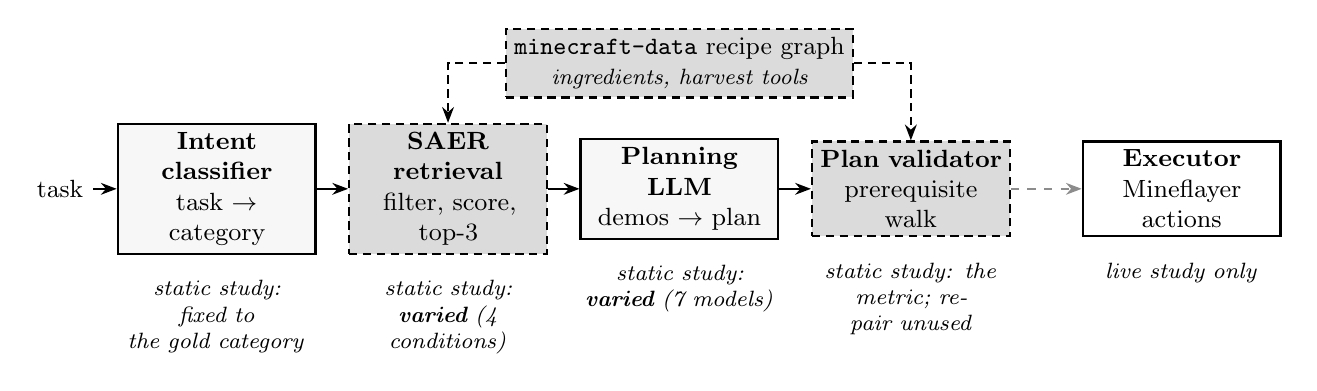
\begin{tikzpicture}[
  node distance=4mm,
  font=\small,
  box/.style={rectangle, draw, thick, align=center, text width=2.3cm,
              minimum height=1.15cm, inner sep=3pt},
  neu/.style={box, fill=black!3},
  sym/.style={box, fill=black!14, densely dashed},
  proc/.style={box, fill=white},
  kb/.style={rectangle, draw, thick, densely dashed, fill=black!14,
             align=center, inner sep=3pt},
  arr/.style={-{Stealth[length=2mm]}, thick},
  off/.style={-{Stealth[length=2mm]}, thick, dashed, black!45},
  tag/.style={font=\footnotesize\itshape, align=center, text width=2.5cm}
]
\node[neu] (intent) {\textbf{Intent classifier}\\ task $\rightarrow$ category};
\node[sym, right=of intent] (saer) {\textbf{SAER retrieval}\\ filter, score, top-3};
\node[neu, right=of saer] (llm) {\textbf{Planning LLM}\\ demos $\rightarrow$ plan};
\node[sym, right=of llm] (val) {\textbf{Plan validator}\\ prerequisite walk};
\node[proc, right=9mm of val] (exec) {\textbf{Executor}\\ Mineflayer actions};
\node[kb, above=5mm of llm] (kb) {\texttt{minecraft-data} recipe graph\\
  {\footnotesize\itshape ingredients, harvest tools}};

\node[anchor=east] (in) at ([xshift=-3mm]intent.west) {task};
\draw[arr] (in) -- (intent);
\draw[arr] (intent) -- (saer);
\draw[arr] (saer) -- (llm);
\draw[arr] (llm) -- (val);
\draw[off] (val) -- (exec);
\draw[arr, densely dashed] (kb.west) -| (saer.north);
\draw[arr, densely dashed] (kb.east) -| (val.north);

\node[tag, below=2mm of intent] {static study: fixed to\\ the gold category};
\node[tag, below=2mm of saer] {static study:\\ \textbf{varied} (4 conditions)};
\node[tag, below=2mm of llm] {static study:\\ \textbf{varied} (7 models)};
\node[tag, below=2mm of val] {static study: the\\ metric; repair unused};
\node[tag, below=2mm of exec] {live study only};
\end{tikzpicture}%
}
\caption{Pipeline, and each component's role in the confirmatory static
study.  Dashed, shaded boxes are symbolic and do not learn: the
\texttt{minecraft-data} recipe graph and the two modules that read it.  The
intent classifier and the planning LLM are LLM calls.  Only the retrieval
condition and the planning model are varied; the task category is supplied
from the benchmark label; the validator acts only as the scorer, and its repair
path and the executor (grey dashed arrow) are exercised only in the live study
(\appref{sec:live}).}
\label{fig:pipeline}
\end{figure}

\noindent\textbf{Why demonstrations rather than the graph.}  The recipe graph
could be handed to the model directly, as Goal-Oriented
Graphs~\citep{leung2025knowledge} do, or to a classical planner, which can
derive a crafting target's prerequisite chain deterministically; the release
contains such a chain resolver on its runtime repair path.  We study
demonstrations for three reasons.  The graph covers only part of the task:
\texttt{minecraft-data} lists crafting recipes but no smelting route (nothing
yields an iron ingot from raw iron) and no tool-tier ordering, and SAER's ingredient term is zero on 18 of the 60
tasks, every gathering and combat task among them (\secref{sec:scoring}).  A demonstration delivers the prerequisites already in
order and in the bot's executable command grammar.  And the agent we build on
receives tasks as free-form chat across categories, for which demonstrations
are the interface it already has.  The LLM is therefore our object of study,
not a competitor to a classical planner.  Supplying each target's resolved chain
is the natural next baseline, and we have not run it.

\subsection{Category Filtering}
\label{sec:catfilter}

The intent classifier (\texttt{getIntent()} in the release) asks the planning
LLM for one label from a fixed set: \texttt{craft}, \texttt{collect},
\texttt{cook}, \texttt{build}, \texttt{combat} and \texttt{explore}, plus a
\texttt{general} fallback.  \texttt{combat} was added \emph{after} the
evaluation runs, when we found the original classifier could not route to the
combat file (\appref{app:intent_oracle}).  Only demonstrations from the file
mapped to the label are admitted as retrieval candidates.  The filter is
motivated by the finding that irrelevant context degrades
reasoning~\citep{shi2023large}, not measured against it: no condition here runs unfiltered.  In the static
evaluation the category is the task's ground-truth label, so retrieval quality
is an \emph{oracle-category upper bound}; the bound is tight here, since the
deployed classifier routes 180/180 trials to the correct file, on one provider
endpoint and 60 templated prompts (\appref{app:intent_oracle}).

\subsection{Composite Scoring}
\label{sec:scoring}

Given a query task $q$ and a candidate example $e$ from the same
category, SAER computes a scalar relevance score $S(q, e) \in [0, 1]$:
\begin{equation}
S(q, e) = \alpha \cdot I(q,e) + \beta \cdot K(q,e) + \gamma \cdot M(q,e) + \delta \cdot L(q,e),
\label{eq:score}
\end{equation}
where $\alpha{+}\beta{+}\gamma{+}\delta{=}1$.  The benchmark uses the
\emph{cold-start} weights $(0.50, 0.35, 0.00, 0.15)$ throughout, for an empty
inventory; a \emph{default} $(0.40, 0.30, 0.20, 0.10)$ for a known inventory
targets mid-task replanning and is not evaluated here.  Cold start sets
$\gamma{=}0$ because $M$ never depends on $q$, so it would act as a standing
preference for low-tier examples rather than a relevance term.  The default's
4:3:2:1 ordering encodes our prior on each dimension's discriminative value
(ingredient overlap first, level only a tiebreaker).  Weights were
fixed before evaluation and no experiment here shows them optimal: on the
frozen benchmark the deployed weights are indistinguishable from uniform
(\appref{app:deployed_ablation}), and an earlier 35-task ablation is silent on
their ordering (\appref{app:weights}).  They are a working point, not a
demonstrated optimum.

All four components take values in $[0,1]$; the first two are Jaccard
overlaps, the last two normalised proximities.
\textbf{Ingredient Overlap ($I$).}  Let $R_q, R_e$ be the crafting
ingredient sets of $q$ and $e$, resolved from the \texttt{minecraft-data}
recipe graph: $I(q,e) = |R_q \cap R_e| / (|R_q \cup R_e| + \varepsilon)$,
$\varepsilon = 10^{-6}$; $I$ is identically zero when either side resolves to no
recipe, which measurement puts at all 16 gathering and combat tasks plus 2 of
the 44 crafting ones; on those 18 the ranking falls to $K$ and $L$ alone.
SAER's increment over BM25 is concentrated in the complement, where
$\alpha{\cdot}I$ can fire (\appref{app:strata}).
\textbf{Keyword Overlap ($K$).}  Let $W_q, W_e$ be content-word sets
(nouns, verbs, item names after stop-word removal):
$K(q,e) = |W_q \cap W_e| / (|W_q \cup W_e| + \varepsilon)$.
\textbf{Mining-Tier Gap ($M$).}  With $t_{\text{req}}(e) \in \{0,1,2,3\}$
the minimum pickaxe tier $e$ requires (0=none, 1=wooden, 2=stone, 3=iron)
and $t_{\text{player}}$ the agent's best tier,
$M = 1 - \max(0,\, t_{\text{req}}(e) - t_{\text{player}})/3$; with
$\gamma{=}0$ it enters no reported number.
\textbf{Level Proximity ($L$).}  Examples carry a hand-annotated
$\ell_e \in \{1,2,3\}$; the query's $\ell_q \in \{1,2,3,4\}$ comes from
surface keywords in the request (default 2), and
$L = 1 - |\ell_q - \ell_e|/3$.  The heuristic never reads the benchmark's tier
label and does not recover it --- it agrees on 20/60 tasks, what a constant
``L2'' guess scores --- so $\delta{\cdot}L$ carries no tier oracle
(\appref{app:intent_oracle}).
How the ranked examples enter the prompt, and why no term in that
construction is learned, is stated in \appref{app:prompt}.

\subsection{Context Assembly}
\label{sec:context}

The top-$k$ candidates ($k{=}3$) are ordered by descending $S(q,e)$,
so the most relevant comes first; the block itself sits mid-prompt,
after the command reference.  Each example is rendered as plain
text, not JSON: \texttt{Step N:}, \texttt{Prerequisites:},
\texttt{Produces:}, then one \texttt{Command:} per bot call; the model is
asked for the same shape with \texttt{Reasoning:} replacing
\texttt{Produces:} --- a step-by-step form after \citet{wei2022chain} and
ReAct~\citep{yao2023react}.

\subsection{Plan Validation}
\label{sec:planval}

The plan validator (\texttt{PlanValidator} in the release) checks a plan's
prerequisite structure over a virtual inventory before any in-game action.
At runtime, on failure, it permits one gap-repair regeneration before
execution (\appref{app:pseudocode}).  In the static study its walk is
reimplemented single-pass and repair-free as the scorer
(\secref{sec:protocol}), so the repair path is exercised only by the live study
(\appref{sec:live}), and every static number, Table~\ref{tab:main} and the
ablation included, measures the unrepaired plan.

% ============================================================
\section{Experiments}

\subsection{Evaluation Tasks}
\label{sec:tasks}

We evaluate on a held-out benchmark of \textbf{60 tasks} spanning three
Minecraft task categories (44 crafting, 11 gathering, 5 combat) and
three difficulty tiers.  No task appears in the demonstration set, verified
by slug-level non-overlap checking after an earlier benchmark revision replaced
24 overlapping tasks.  The benchmark and training data were frozen before any
model evaluation began, and no task was added or removed after seeing model
outputs.  Residual structural overlap is modest.  For the 44
crafting tasks the symmetric ingredient Jaccard to the nearest demonstration
has mean 0.188 (0.290 on a later corrected bank) and never exceeds 0.333 on
the bank the runs retrieved over; no gathering task's goal item is the final
product of any demonstration, whereas the same check flags all five combat
tasks (\secref{sec:combat_design}).  On the evaluation-time bank the gain
rises with overlap, but the direction reverses on the corrected bank, and the
high-overlap stratum is the iron- and stone-tier multi-hop chains, so overlap
is substantially a proxy for prerequisite depth and neither panel points to
near-copies (\appref{app:overlap}).

\textbf{L1} (20 tasks): single-material tasks achievable with basic
tools (\texttt{wooden\_sword}, \texttt{chest}, \texttt{bowl}).
\textbf{L2} (20 tasks): two-chain tasks typically culminating
in iron-tool use (\texttt{iron\_axe}, \texttt{cauldron},
\texttt{hopper}); L2 is the primary discrimination tier because it
requires the complete wooden$\to$stone$\to$iron pickaxe chain.
\textbf{L3} (20 tasks): three-or-more-chain tasks involving deep
dependency trees (\texttt{compass}, \texttt{golden\_pickaxe},
\texttt{anvil}).

\subsection{Models and Conditions}
\label{sec:models}

We evaluate seven models from five organisations (\appref{app:models}): five
primary-study models under \texttt{no\_retrieval} and \texttt{saer\_cold},
and a two-model open-weight replication panel (Gemma4-26B/31B) outside the
pre-specified test family.  Four retrieval conditions are compared on
Qwen2.5-Max, the ablation model.  Sampling temperature is 0.7 for Qwen3-8B,
GPT-4o and Claude Sonnet~4.5, the value in the harness's evaluation profiles,
not tuned on this benchmark.  The Qwen2.5-Max, DeepSeek-V3 and Gemma4 requests
set no temperature, so those endpoints used their server defaults, which the
run files do not record (\appref{app:models}).  Every within-model
comparison, and so every retrieval effect, keeps the model and its setting
fixed; levels across models, and the three cross-model tests of the family,
mix settings.

\noindent\textbf{Conditions.}
\begin{itemize}\setlength\itemsep{1pt}
  \item \textbf{no\_retrieval}: No retrieved examples; the task and the shared rule text only
  (\appref{app:prompt}).
  \item \textbf{saer\_cold}: SAER with cold-start weights
  $(\alpha,\beta,\gamma,\delta){=}(0.50,0.35,0.00,0.15)$; agent
  inventory treated as empty.
  \item \textbf{random\_retrieval} (Qwen2.5-Max ablation only): Three
  examples selected uniformly at random from the same-category training
  set.
  \item \textbf{bm25\_retrieval} (Qwen2.5-Max ablation \emph{and}
  evaluated cross-model on all five primary-study models, \secref{sec:ablation}): Okapi
  BM25~\citep{robertson2009probabilistic} ($k_1{=}1.5$, $b_L{=}0.75$;
  $b_L$ is BM25's length-normalisation term, not McNemar's $b$).
\end{itemize}

\subsection{Evaluation Protocol}
\label{sec:protocol}

\textbf{Static plan evaluation.}  For each task and condition the planning
LLM writes a plan, which is scored offline without a live bot: the validator
walks the plan's commands (\texttt{collectBlocks}, \texttt{craftRecipe},
\texttt{smeltItem}) over a virtual inventory that starts empty (pseudocode in
\appref{app:pseudocode}).  Each condition is run with three seeds; a task
passes if it passes in at least two (\textbf{majority vote}).

\textbf{Metrics.}  The primary metric is the \emph{Strict Plan Pass Rate}
(SPR; labelled TCR, for task completion rate, in the released scripts\footnote{Appendices, code and data: \url{https://github.com/Jayden23018/existence-before-relevance}}): the fraction of tasks whose plan
has no prerequisite gap in the inventory walk and ends with the goal item
present.  SPR measures the prerequisite-structure validity of a plan, not task
completion.  \emph{Plan Validity Rate} (PVR) checks only \emph{explicitly
declared} preconditions and the goal item, not implicit tool-tier
requirements, so the gap PVR$-$SPR separates structural failures from
detail-level ones.

\textbf{Two scorings.}  The pre-specified scorer credits each produced item
but never debits consumed ones, on the rationale that quantities are the
executor's job; an item produced once satisfies every later requirement.  We
therefore also report a \emph{debited} SPR, which charges each craft and smelt
so that every produced unit is spent once (\appref{app:exposure}).  The
leniency is not symmetric: on Qwen2.5-Max, debiting removes 0 of
\texttt{no\_retrieval}'s 19 passes but 7 of random's 38, 14 of BM25's 42 and
16 of SAER's 49, because a scorer that never debits can only over-credit plans
that produce things, and retrieval makes plans produce more.  Credit-only
remains the confirmatory scorer, since the test family was fixed for it;
debited figures appear beside it in Tables~\ref{tab:main}
and~\ref{tab:ablation}.  Against the published Plancraft oracle the scorer
agrees on 95.8\% of 11,177 craft invocations ($\kappa{=}0.753$).  That
certifies single-craft feasibility only: one issue class of six, not the
tool-gap class behind two models' failures (\appref{app:plancraft}).

\textbf{Re-validation.}  Two harness defects were found after generation: a
missing recipe-resolver hook that disabled three of SAER's scoring dimensions,
and a missing mining-drop alias in the scorer.  Every \texttt{saer\_cold} arm in Table~\ref{tab:main}
was regenerated after the fix, so each is a later run than its
\texttt{no\_retrieval} arm, and every stored seed plan of every condition was
then re-scored with one fixed validator.  All confirmatory SPR, PVR and
McNemar values come from that pass (\appref{app:provenance}); three
exploratory panels quote runtime verdicts beside re-scored ones
(\appref{app:livecombat}, \appref{app:capacity}, \appref{app:thinking}).

\textbf{Statistical testing.}  McNemar's exact binomial
test~\citep{mcnemar1947note} on per-task majority-vote outcomes,
$\alpha{=}0.05$, Bonferroni-corrected over 13 pre-specified tests (5
per-model $+$ 5 ablation $+$ 3 cross-model): $\alpha'{=}0.0038$.  We call a
result \emph{family-wise significant} if $p{<}\alpha'$, \emph{nominal} if
$0.0038{\le}p{<}0.05$, and \emph{not significant} otherwise; every headline
verdict is a Bonferroni verdict.  The uniformly more powerful Holm
step-down~\citep{holm1979simple} over the same 13 tests is reported post hoc
as a labelled sensitivity analysis (Holm rejects 11, Bonferroni 9;
\appref{app:mcnemar}).  The Gemma4 panel lies outside the family and is
reported descriptively.  The 55 demonstrations (25 crafting, 21
collecting, 9 combat) were AI-drafted from hand-written seeds and hand-checked
(\appref{app:traindata}).

\subsection{Combat Subgroup}
\label{sec:combat_design}

The five combat tasks (L1--L3) are part of the 60 and counted in
Table~\ref{tab:main}, so they form a within-benchmark subgroup, not a
hold-out.  Five of the nine combat demonstrations target the same five mobs
and differ only by slug prefix (\texttt{combat/creeper} vs.\
\texttt{combat/kill\_creeper}), which the slug-level check misses; the runs
behind Table~\ref{tab:main} retrieve over them (\appref{app:nocombat} bounds
what that costs).  A separate probe re-runs the five tasks on Qwen2.5-Max under
all four conditions without those five demonstrations, over a combat pool with acquisition chains
corrected for a cold start (\appref{app:livecombat}).

% ============================================================
\section{Results}

\subsection{Main Results}
\label{sec:mainresults}

\begin{table}[tbp]
\caption{Cross-architecture results (60 tasks, 3-seed majority vote).  SPR
under the pre-specified credit-only scorer and under debiting
(\secref{sec:protocol}); PVR and the L1--L3 tier counts (of 20 each) are credit-only.
\textbf{L2} is the discrimination tier.  Gap $=$ PVR$-$SPR in tasks.  $\Delta$
$=$ \texttt{saer\_cold} minus \texttt{no\_ret} (\texttt{no\_retrieval}), differencing the rounded
percentages, with McNemar exact $p$; \textbf{bold} $=$ below
$\alpha'{=}0.0038$.  $^\ddagger$ $=$ 4B active parameters (Mixture-of-Experts).  The
replication panel lies outside the pre-specified family.  Verdicts in
\appref{app:mcnemar} and \appref{app:exposure}; run provenance in
\appref{app:provenance}; denominator sensitivity in \appref{app:denom}.}
\label{tab:main}
\footnotesize\setlength{\tabcolsep}{3pt}\renewcommand{\arraystretch}{0.9}
\centering
\begin{tabular}{llrrrrrrrll}
\toprule
& & \multicolumn{2}{c}{SPR (/60)} & & & & & & \multicolumn{2}{c}{SAER $\Delta$ (pp)} \\
\cmidrule(lr){3-4}\cmidrule(lr){10-11}
Model & Cond. & credit & debited & PVR & Gap & L1 & \textbf{L2} & L3 & credit & debited \\
\midrule
Qwen3-8B       & no\_ret    & 14 (23\%) & 13 (22\%) & 47 & +33 & 9  & 3  & 2  & --- & --- \\
Qwen3-8B       & saer\_cold & 26 (43\%) & 24 (40\%) & 48 & +22 & 12 & 11 & 3  & +20 ($p{=}0.0075$) & +18 ($p{=}0.0127$) \\
\addlinespace
GPT-4o         & no\_ret    & 23 (38\%) & 20 (33\%) & 29 & +6  & 17 & 3  & 3  & --- & --- \\
GPT-4o         & saer\_cold & 41 (68\%) & 34 (57\%) & 46 & +5  & 17 & 16 & 8  & \textbf{+30} ($p{<}0.001$) & \textbf{+24} ($p{<}0.001$) \\
\addlinespace
Claude S.~4.5  & no\_ret    & 25 (42\%) & 22 (37\%) & 29 & +4  & 19 & 4  & 2  & --- & --- \\
Claude S.~4.5  & saer\_cold & 51 (85\%) & 35 (58\%) & 57 & +6  & 20 & 13 & 18 & \textbf{+43} ($p{<}0.001$) & \textbf{+21} ($p{<}0.001$) \\
\addlinespace
Qwen2.5-Max    & no\_ret    & 19 (32\%) & 19 (32\%) & 28 & +9  & 17 & 2  & 0  & --- & --- \\
Qwen2.5-Max    & saer\_cold & 49 (82\%) & 33 (55\%) & 56 & +7  & 20 & 14 & 15 & \textbf{+50} ($p{<}0.001$) & \textbf{+23} ($p{<}0.001$) \\
\addlinespace
DeepSeek-V3    & no\_ret    & 33 (55\%) & 25 (42\%) & 41 & +8  & 17 & 6  & 10 & --- & --- \\
DeepSeek-V3    & saer\_cold & 52 (87\%) & 35 (58\%) & 55 & +3  & 19 & 17 & 16 & \textbf{+32} ($p{<}0.001$) & +16 ($p{=}0.0309$) \\
\midrule
\multicolumn{11}{l}{\emph{Replication panel (outside the pre-specified Bonferroni family)}} \\
\addlinespace[2pt]
Gemma4-26B$^{\ddagger}$ & no\_ret    & 44 (73\%) & 35 (58\%) & 53 & +9  & 18 & 12 & 14 & --- & --- \\
Gemma4-26B$^{\ddagger}$ & saer\_cold & 48 (80\%) & 28 (47\%) & 58 & +10 & 17 & 16 & 15 & +7 ($p{=}0.388$) & $-$11 ($p{=}0.118$) \\
\addlinespace
Gemma4-31B & no\_ret    & 46 (77\%) & 37 (62\%) & 53 & +7  & 18 & 13 & 15 & --- & --- \\
Gemma4-31B & saer\_cold & 53 (88\%) & 37 (62\%) & 58 & +5  & 19 & 17 & 17 & +11 ($p{=}0.0156$) & 0 ($p{=}1.000$) \\
\bottomrule
\end{tabular}
\renewcommand{\arraystretch}{1}
\end{table}

\noindent\textbf{Finding~1: an L2 bottleneck in five of seven models.}  The
five primary-study models score 10--30\% on L2 without retrieval (median
15\%; a 2$\times$5 homogeneity test does not reject, $p{=}0.539$) against
45--95\% on L1 (median 85\%).  The Gemma4 replication panel already clears
60--65\% on L2 without retrieval, so the diagnosis applies to the five primary
models, not to every model we ran.  We have no tested explanation for the difference.

\noindent\textbf{Finding~2: retrieval helps all five, the 8B model
included.}  SAER improves all five primary models by $+$20 to $+$50\,pp, four
family-wise significantly; Qwen3-8B gains least ($+$20\,pp, $p{=}0.0075$:
Holm yes, Bonferroni no).  Under debiting all five gains stay positive
($+$16 to $+$24\,pp) and three clear $\alpha'$.  Gain does not track parameter
count (DeepSeek-V3, 671B, gains less than Qwen2.5-Max), and two of five sizes are undisclosed and a third only approximate
(\appref{app:models}), so we make no capacity-scaling claim.  Qwen3-8B keeps
the largest PVR$-$SPR gap ($+$22 vs.\ $+$3 to $+$7): given correct templates it
still mis-specifies counts (2 iron ingots for a helmet needing 5), a residual
distinct from the bottleneck.  Of the five, DeepSeek-V3 alone reaches 10/20 at L3 without
retrieval (others 0--3/20); with SAER it converges with Qwen2.5-Max
overall ($p{=}0.453$).  On the replication panel the credit-only gains
($+$7 and $+$11\,pp) do not survive debiting.

\noindent\textbf{The L2 tier.}  L2 recovery spans $+$40 to $+$65\,pp, again
non-monotone in parameter count.  On Qwen2.5-Max random retrieval alone lifts
L2 from 10\% to 70\%, and \texttt{saer\_cold} reaches the same 14/20, so L2
does not separate SAER from random; BM25 trails both there (11/20) but leads
random at L3 (14/20 vs.\ 7/20).  As BM25 and random do not differ overall
($p{=}0.424$), we read neither tier split as more than noise (per-tier counts
in \appref{app:perseed}).

\subsection{Qwen2.5-Max Four-Condition Ablation}
\label{sec:ablation}

\begin{table}[htbp]
\vspace{-8pt}
\caption{Four-condition ablation on Qwen2.5-Max (60 tasks, 3-seed majority
vote) under both scorings.  $\Delta$ is against \texttt{no\_retrieval}, or
between the two named arms, differencing rounded percentages; 95\% CI on the
paired difference~\citep{newcombe1998improved}, credit-only.  $b/c$ $=$
tasks passed only by the condition (or first-named arm) / only by the
comparator, with McNemar exact $p$.}
\label{tab:ablation}
\footnotesize\setlength{\tabcolsep}{4pt}
\centering
\begin{tabular}{lrrllrll}
\toprule
& \multicolumn{4}{c}{Credit-only (pre-specified)} & \multicolumn{3}{c}{Debited} \\
\cmidrule(lr){2-5}\cmidrule(lr){6-8}
Condition & SPR & PVR & $\Delta$ [95\% CI] & $b/c$ ($p$) & SPR & $\Delta$ & $b/c$ ($p$) \\
\midrule
no\_retrieval & 19 & 28 & --- & --- & 19 & --- & --- \\
random        & 38 & 54 & $+$31 [19, 42] & 19/0 (${<}0.001$) & 31 & $+$20 & 13/1 (0.0018) \\
BM25          & 42 & 53 & $+$38 [24, 50] & 24/1 (${<}0.001$) & 28 & $+$15 & 12/3 (0.0352) \\
saer\_cold    & 49 & 56 & $+$50 [36, 61] & 30/0 (${<}0.001$) & 33 & $+$23 & 15/1 (${<}0.001$) \\
\midrule
BM25 vs.\ random   & & & $+$7 [$-$5, 18] & 9/5 (0.424)  & & $-$5 & 1/4 (0.375) \\
SAER vs.\ BM25     & & & $+$12 [3, 20]   & 7/0 (0.0156) & & $+$8 & 6/1 (0.125) \\
\bottomrule
\end{tabular}
\end{table}

\noindent(1)~\textbf{Existence is the primary lever.}  The step from no
retrieval to random same-category demonstrations is the largest one
($+$31\,pp; $+$20\,pp debited, $b{=}13$, $c{=}1$, $p{=}0.0018$), family-wise
significant under both scorings.  The step adds same-category worked examples to a rule text that already states
the output format and one generic chain.  Random demonstrations carry the same step grammar as SAER's (\secref{sec:context}), so part of this may be exposure to
format rather than to procedural content, in line with format effects on
classification tasks~\citep{min2022rethinking}; no condition here separates the two.  The combat
subgroup agrees: re-run without its five near-duplicate demonstrations, no
retrieval reaches 0/5 and every retrieval condition 3/5 or better, too few
tasks to rank the variants (\appref{sec:combat_probe}).

\noindent(2)~\textbf{Relevance is directional, not established.}  SAER over
BM25 gives $b{=}7$, $c{=}0$, $p{=}0.0156$, $+$12\,pp [95\% CI $+$3, $+$20].
Four qualifications bound it.  \emph{Power:} with seven discordant tasks the
smallest attainable two-sided $p$ is $2\cdot0.5^{7}{=}0.0156$, so the
Bonferroni bar (which needs $b{+}c{\ge}10$) was out of reach whatever the
outcome; post hoc Holm clears it at the pre-specified family size $m{=}13$
and fails at $m{=}14$ (\appref{app:mcnemar}).  \emph{Scorer:} debiting
reduces it to $b{=}6$, $c{=}1$, $p{=}0.125$, and BM25 (28) falls below random
(31).  \emph{Generation epoch:} Qwen2.5-Max's BM25 arm was generated 16 days
before its SAER arm on a provider alias, not a date-pinned identifier, so an
endpoint change is a rival explanation that re-scoring cannot remove
(\appref{app:provenance}).  \emph{Replication:} across the five primary models
SAER beats BM25 on four (nominally on two) and trails by one task on GPT-4o;
the one-sided 4--1 sign test gives $p{=}0.188$, and six of the seven discordant tasks lie in the 42
where ingredient overlap is non-zero (\appref{app:strata}).  One check
cuts the other way: SAER is handed the \emph{more} defective demonstrations
(top-1 materially short on 22/60 tasks vs.\ BM25's 8/60, $p{=}0.00012$) and
still scores higher, so demonstration quality does not explain its edge
(\appref{app:exposure}).  We read relevance as a consistent but unconfirmed
increment.

% ============================================================
\section{Analysis and Discussion}

\subsection{Why L2 Fails, and What Demonstrations Transmit}
\label{sec:knowledge_gap}

The L2 wall holds with the tool chain stated in the rule text, and it does not
track scale.  Counting the
scorer's typed issues over every no-retrieval failure
(\appref{app:failmodes}), 20--41 of each primary model's 27--46 failing tasks
(74--95\%) carry an \emph{unacquired prerequisite}: a declared precondition, a
craft ingredient or a tool never obtained.  The signature is shared, its
composition is not: ingredient gaps run 39 tasks on Qwen3-8B against 3 on
GPT-4o, and tool gaps 33 on Qwen2.5-Max against 2 on Claude Sonnet~4.5, so we
claim no common failure profile, and the version-specific naming check fires
on no failure in the primary study (the rule text states the drop names).  Correctness binds on one exploratory
contrast: on a superseded 35-task benchmark six L2 demonstrations declared a
stone pickaxe they never crafted, and under one scorer SAER read 1/13 at L2
against random's 6/13; the post-repair reading (11--12/13) is confounded with
two concurrent validator fixes, and the episode predates every run reported
here (\appref{app:weights}).

\textbf{Defects are inherited verbatim.}  The mechanism behind that contrast
is measurable on the frozen runs.  All nine combat demonstrations use
\texttt{!equipItem}, which is not in the bot's command registry
(\texttt{!equip} is).  Across every stored combat-task plan, superseded runs
included, the string appears in 0 of 505 trials without retrieval and in 726
of 1,016 with it (71.5\%; 72.9\% under SAER, 74.2\% BM25, 61.2\% random): the
models never invent the command and copy it about three times in four once
shown it (\appref{app:intent_oracle}).  Quantities travel the same way.  Nine
of the collecting bank's 17 \texttt{oak\_planks} calls ask for 4, too few for
a crafting table, sticks and a pickaxe.  On the 11 gathering tasks four of the
five models never emit 4 without retrieval (the rule text's chain shows 12), yet under SAER they do in 10 of 12
trials on Qwen2.5-Max, 4 of 15 on DeepSeek-V3 and 2 of 17 on GPT-4o, while
Claude Sonnet~4.5 overrides the demonstration every time (Qwen3-8B emits 4
under both conditions; \appref{app:quantity}).  Neither defect moves a
credit-only number, since that scorer credits no equip step and charges no
quantity, which is why both survived to be found.

\subsection{Limitations}
\label{sec:limits}

\noindent\textbf{Scope.}  Beyond the offline scope stated in \secref{sec:intro}, the live study (126 trials on DeepSeek-V3) floors both conditions at 2/21 L2
trials because execution-framework failures dominate, so it neither
corroborates nor contradicts the static result (\appref{sec:live}).  The
cross-agent study (\appref{app:crossagent}) probes a different retrieval stage
and carries no claim.  \textbf{Metric.}  Credit-only SPR over-credits the retrieval arms more than
the baseline (\secref{sec:protocol}); scoring is automated and unblinded; and
McNemar on majority-vote outcomes models neither task difficulty nor
model$\times$condition interaction.

\noindent\textbf{Relevance evidence.}  One pre-specified test on one model, seven
discordant tasks and a 16-day generation gap on a provider alias; settling it
needs a same-window re-run, which we have not done.  The category filter is in
every retrieval condition, so its own contribution is unmeasured.  \textbf{Controls not run.}  We ablate retrieval \emph{policy}, not demonstration
\emph{surface form}: format-only and content-masked controls, and supplying each target's resolved chain, are future work.

\noindent\textbf{Models and decoding.}  Temperature differs across models
(\secref{sec:models}); two primary models used date-pinned identifiers, and the
other three are provider aliases, so endpoint updates between their arms cannot
be excluded.  Three further 8--12B models, run at provider
defaults, keep SAER ceilings at 7/26/34 of 60 when re-scored (7/23/33 at runtime), below the four frontier primary
models (41--52/60) but not all below Qwen3-8B's 26/60, so we claim no
capacity threshold (\appref{app:capacity}).  Without \texttt{minecraft-data} SAER keeps only keyword and level, as on
18/60 tasks already (\appref{app:strata}).

% ============================================================
\section{Conclusion}
\label{sec:conclusion}

Five of the seven LLM planners we tested pass only 10--30\% of two-chain tasks
without retrieval; in 74--95\% of those failures a prerequisite is never acquired
(\secref{sec:knowledge_gap}).  Given a shared rule text, the primary lever is the \emph{existence} of a
same-category demonstration ($+$31\,pp on Qwen2.5-Max; $+$20\,pp debited).
\emph{Relevance} adds an increment that neither its discordance budget nor the
stricter scorer confirms, concentrated in the 42 tasks with ingredient overlap;
on \emph{capacity}, the 8B model gains too.  Demonstrations are inherited, errors
included, so their \emph{correctness} is the next lever, a natural target for
verifiable-reward RL~\citep{zeng2025rlve}.

% ============================================================
\clearpage
% NeurIPS 2026 instructions: "References follow the acknowledgments in the
% camera-ready paper"; pages holding them do not count as content pages.
\begin{ack}
This work received no external funding.  The authors declare no competing
interests.
\end{ack}

\bibliographystyle{plainnat}
\bibliography{references}

\end{document}
